\section{Cronograma}

Realizamos un cronograma tentativo de la totalidad del trabajo, incluyendo el desarrollo de cada caso de uso, el despliegue en cada ecosistema y su documentación asociada.

Cada caso de uso incluye una etapa de \textit{Discovery} en la cuál definiremos su alcance y lo desglosaremos en tareas más concretas.

\begin{figure}[H]
    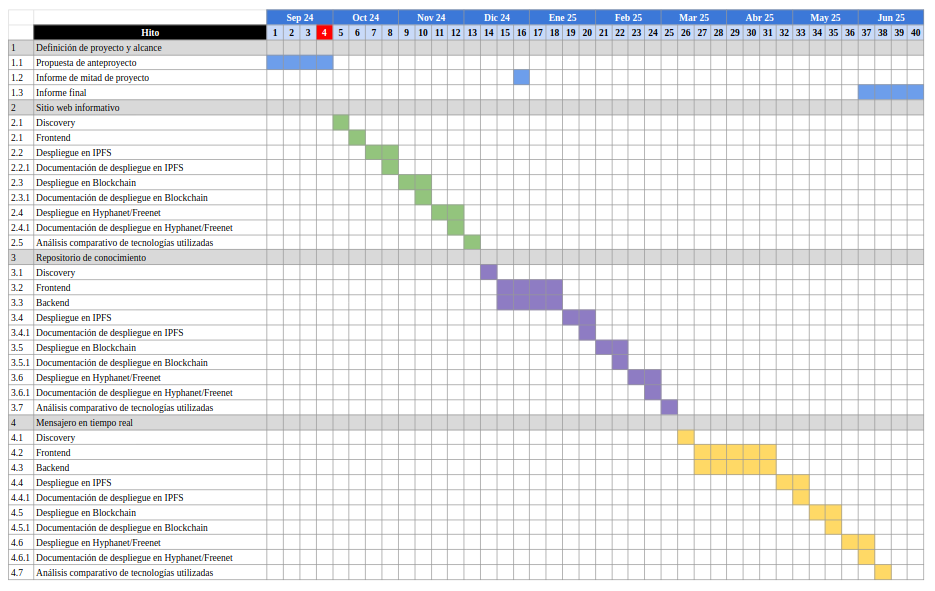
\includegraphics[width=1\linewidth]{img/cronograma.png}
    \caption{Cronograma tentativo}
    \label{fig:enter-label}
\end{figure}

\begin{figure}[H]
    \centering
    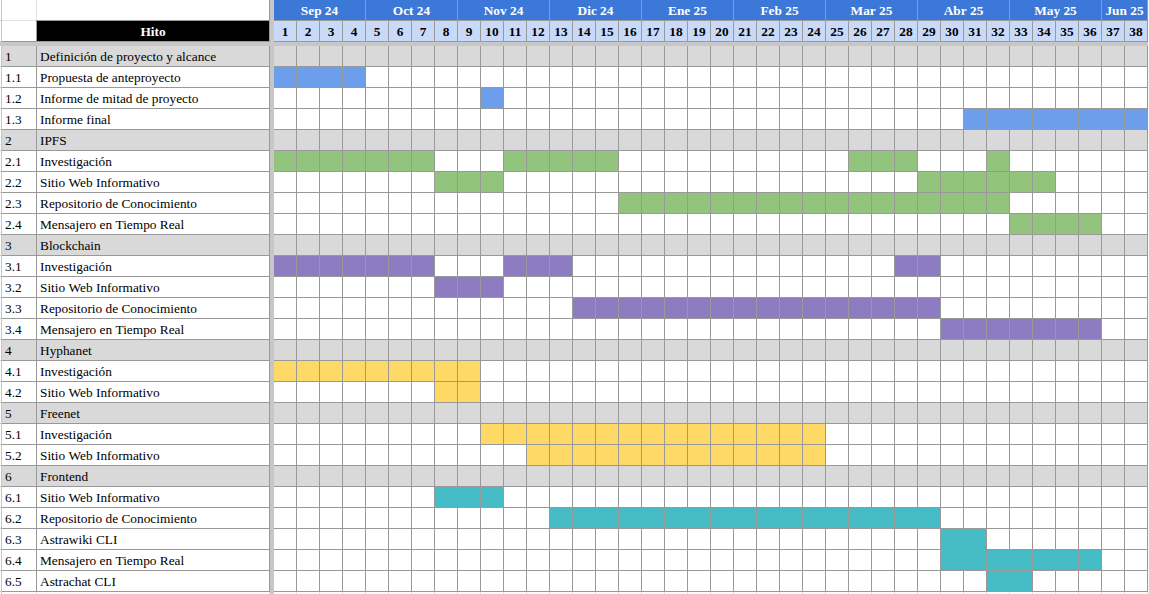
\includegraphics[width=1\linewidth]{img/cronograma-real.png}
    \caption{Cronograma real}
    \label{fig:enter-label}
\end{figure}

\begin{enumerate}

    \item \textbf{Definición de proyecto y alcance}
    \begin{enumerate}[label*=\arabic*.]
        \item Propuesta de anteproyecto (Semanas 1 a 4)
        \item Informe de mitad de proyecto (Semanas 16 a 17)
        \item Informe final (Semanas 37 a 40)
    \end{enumerate}
    
    \item \textbf{Sitio web informativo} (Semanas 5 a 13)
    \begin{enumerate}[label*=\arabic*.]
        \item Discovery
        \item Frontend
        \item Despliegue en IPFS
        \begin{enumerate}[label*=\arabic*.]
            \item Documentación de despliegue en IPFS
        \end{enumerate}
        \item Despliegue en Blockchain
        \begin{enumerate}[label*=\arabic*.]
            \item Documentación de despliegue en Blockchain
        \end{enumerate}
        \item Despliegue en Hyphanet/Freenet
        \begin{enumerate}[label*=\arabic*.]
            \item Documentación de despliegue en Hyphanet/Freenet
        \end{enumerate}
        \item Análisis comparativo de tecnologías utilizadas
    \end{enumerate}
    
    \item \textbf{Repositorio de conocimiento} (Semanas 14 a 25)
    \begin{enumerate}[label*=\arabic*.]
        \item Discovery
        \item Frontend
        \item Backend
        \item Despliegue en IPFS
        \begin{enumerate}[label*=\arabic*.]
            \item Documentación de despliegue en IPFS
        \end{enumerate}
        \item Despliegue en Blockchain
        \begin{enumerate}[label*=\arabic*.]
            \item Documentación de despliegue en Blockchain
        \end{enumerate}
        \item Despliegue en Hyphanet/Freenet
        \begin{enumerate}[label*=\arabic*.]
            \item Documentación de despliegue en Hyphanet/Freenet
        \end{enumerate}
        \item Análisis comparativo de tecnologías utilizadas
    \end{enumerate}
    
    \item \textbf{Mensajero en tiempo real} (Semanas 26 a 38)
    \begin{enumerate}[label*=\arabic*.]
        \item Discovery
        \item Frontend
        \item Backend
        \item Despliegue en IPFS
        \begin{enumerate}[label*=\arabic*.]
            \item Documentación de despliegue en IPFS
        \end{enumerate}
        \item Despliegue en Blockchain
        \begin{enumerate}[label*=\arabic*.]
            \item Documentación de despliegue en Blockchain
        \end{enumerate}
        \item Despliegue en Hyphanet/Freenet
        \begin{enumerate}[label*=\arabic*.]
            \item Documentación de despliegue en Hyphanet/Freenet
        \end{enumerate}
        \item Análisis comparativo de tecnologías utilizadas
    \end{enumerate}

\end{enumerate}

% TODO: agregar cronograma real / explicar en qué se desvió del plan original